\chapter{Despliegue y aplicación web}

Tras los pasos realizados del ciclo de vida de la ciencia de datos (análisis exploratorio, preprocesamiento, modelado y evaluación), en este capítulo se describe el resultado del último paso: el \textbf{despliegue} del modelo final entrenado obtenido para su uso por los usuarios.

\begin{figure}[h]
	\vspace{-6mm}
	\centering
	\makebox[\textwidth][c]{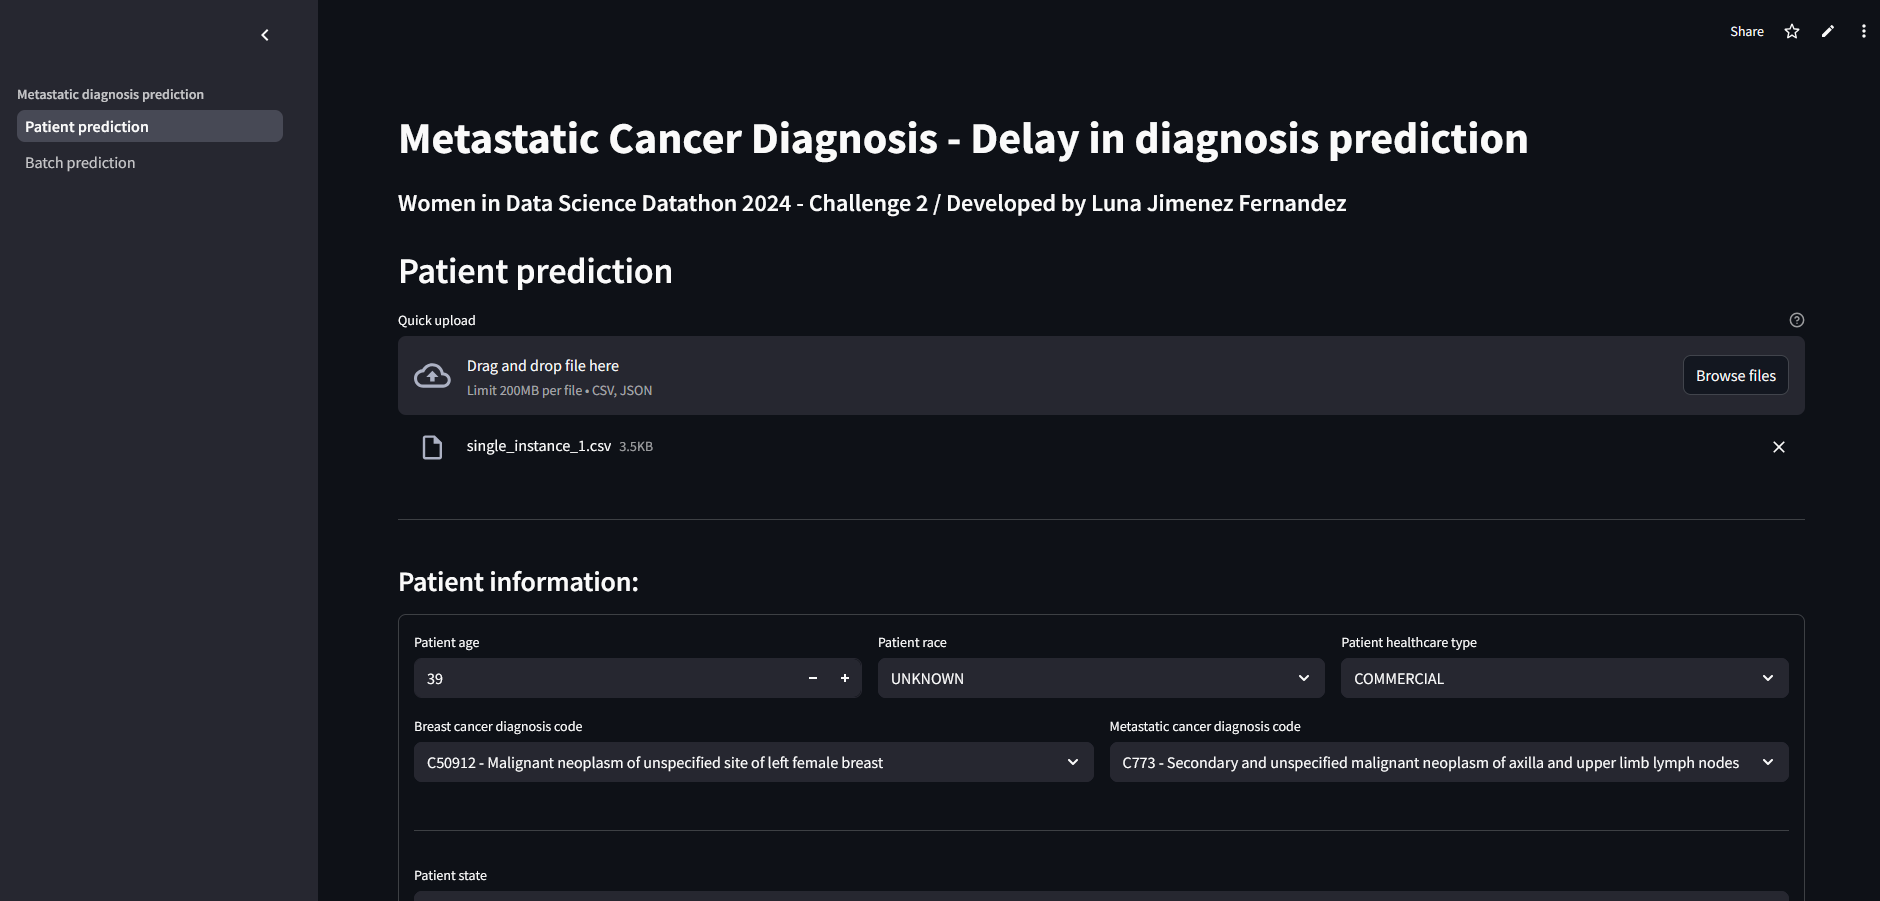
\includegraphics[width=0.7\linewidth]{figs/chapter6/mainwebpage}}
	\captionsetup{belowskip=-20pt, justification=centering}
	\caption{Página principal de la aplicación web}
	\label{fig:ch6main}
\end{figure}

El despliegue se ha realizado a través de una \textbf{aplicación web}, cuyo aspecto se puede observar en la \textbf{Figura \ref{fig:ch6main}}. Esta aplicación es un \textbf{producto mínimo viable} desarrollado a través de \textit{Streamlit} --- una librería de Python para prototipado de aplicaciones---, funcionando mediante un \textbf{modelo embebido} incrustado directamente en la página web. 

Esta aplicación se encuentra disponible en el enlace \url{https://cidaen-m5-thesis-lunajimenezfernandez.streamlit.app/}, teniendo \textbf{dos} funcionalidades principales.


\vspace*{-4mm}
\section{Aplicación para usuario: predicción individual}

La funcionalidad principal de la aplicación es la \textbf{predicción individual del tiempo de diagnóstico}, como se puede observar en la \textbf{Figura \ref{fig:ch6single}}.

\begin{figure}[h]
	\vspace{-3mm}
	\centering
	\makebox[\textwidth][c]{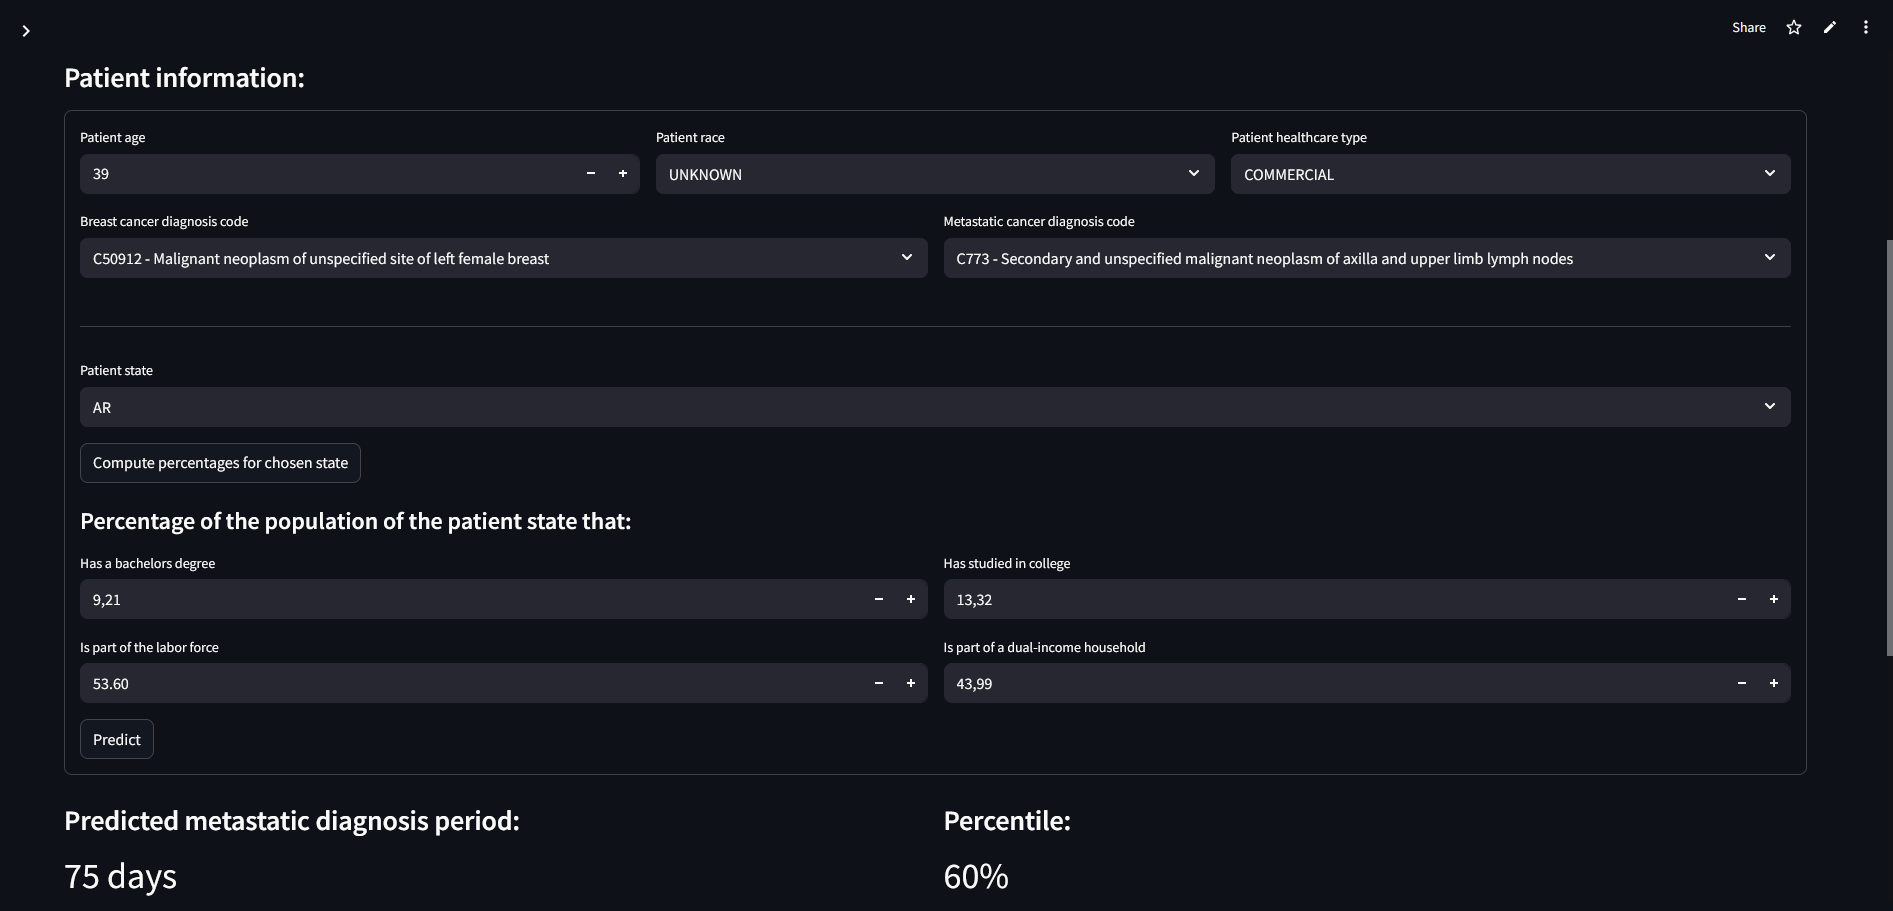
\includegraphics[width=0.7\linewidth]{figs/chapter6/webpageprediction}}
	\captionsetup{belowskip=-25pt, justification=centering}
	\caption{Predicción de tiempo de diagnóstico individual}
	\label{fig:ch6single}
\end{figure}

La aplicación permite introducir manualmente los valores de los \textbf{10 atributos} para obtener de forma automática una predicción del tiempo de diagnóstico de cáncer metastásico para un paciente. Para simplificar la tarea de introducción de datos, se ofrecen las siguientes facilidades:

\begin{itemize}[parsep=1pt, itemsep=1pt, topsep=2pt]
	\item Se incluye una \textbf{descripción completa} de todos los códigos de diagnóstico y la posibilidad de buscar por descripción.
	\item Se incluye opción para introducir automáticamente toda la información del paciente a partir de un fichero \textit{JSON} o \textit{CSV}.
	\item No es factible asumir que un doctor va a conocer la información socioeconómica de la región de sus pacientes, por los que se incluye un botón \textbf{"Compute percentages for chosen state"} que calcula automáticamente los valores para el estado actual.
\end{itemize}

\vspace*{-6mm}
\section{Aplicación \textit{batch}: predicción en bloque}

La segunda funcionalidad ofrecida por la aplicación es la \textbf{predicción de tiempos de diagnóstico en bloque}, como se puede observar en la \textbf{Figura \ref{fig:ch6batch}}.

\begin{figure}[h]
	\vspace{-5mm}
	\centering
	\makebox[\textwidth][c]{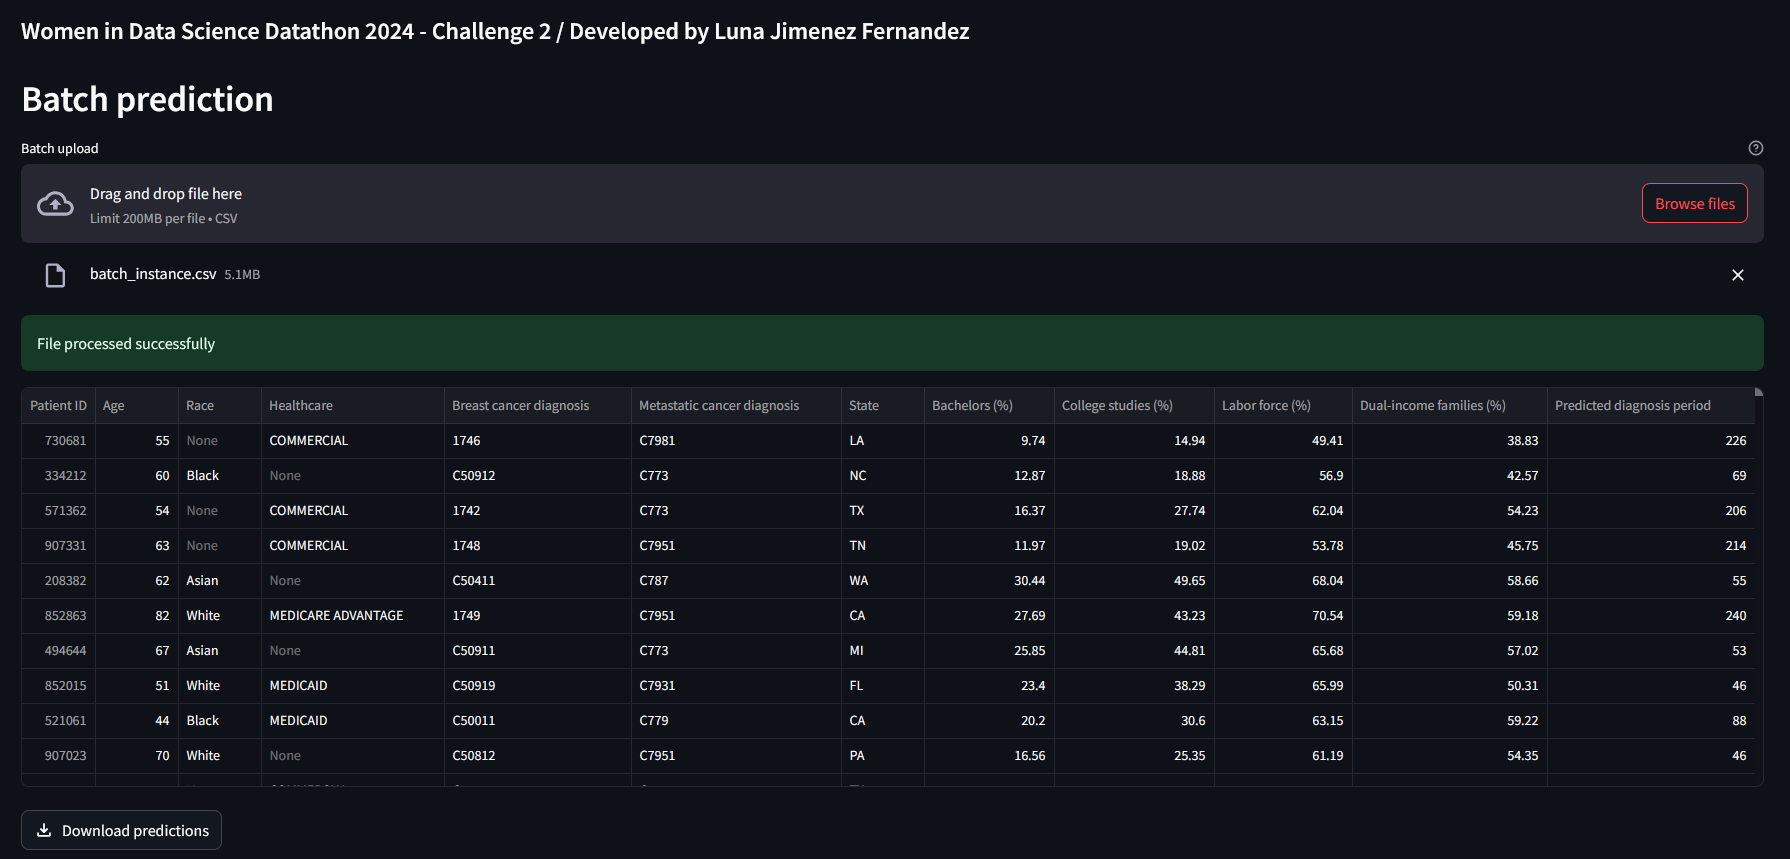
\includegraphics[width=0.7\linewidth]{figs/chapter6/batchprediction}}
	\captionsetup{belowskip=-25pt, justification=centering}
	\caption{Predicción de tiempo de diagnóstico en bloque}
	\label{fig:ch6batch}
\end{figure}

El funcionamiento está más enfocado a la automatización del diagnóstico de un gran número de pacientes, introduciendo un \textbf{fichero CSV} con los datos clínicos relevantes y generando de forma automática la predicción para todos los pacientes. Esta predicción puede ser descargada posteriormente a través del botón \textbf{"Download Predictions"}.